\documentclass[tikz, border=10mm]{standalone}


\newcommand{\track}[2]{%
  \begin{scope}[scale=#2]
 \draw [#1] plot [smooth cycle, tension=2] coordinates {(-0.5, 0) (-1, -1) (0,-1) (1,-1) (0.5, 0) (1, 1) (-1,1)};
\end{scope}} 

\begin{document}
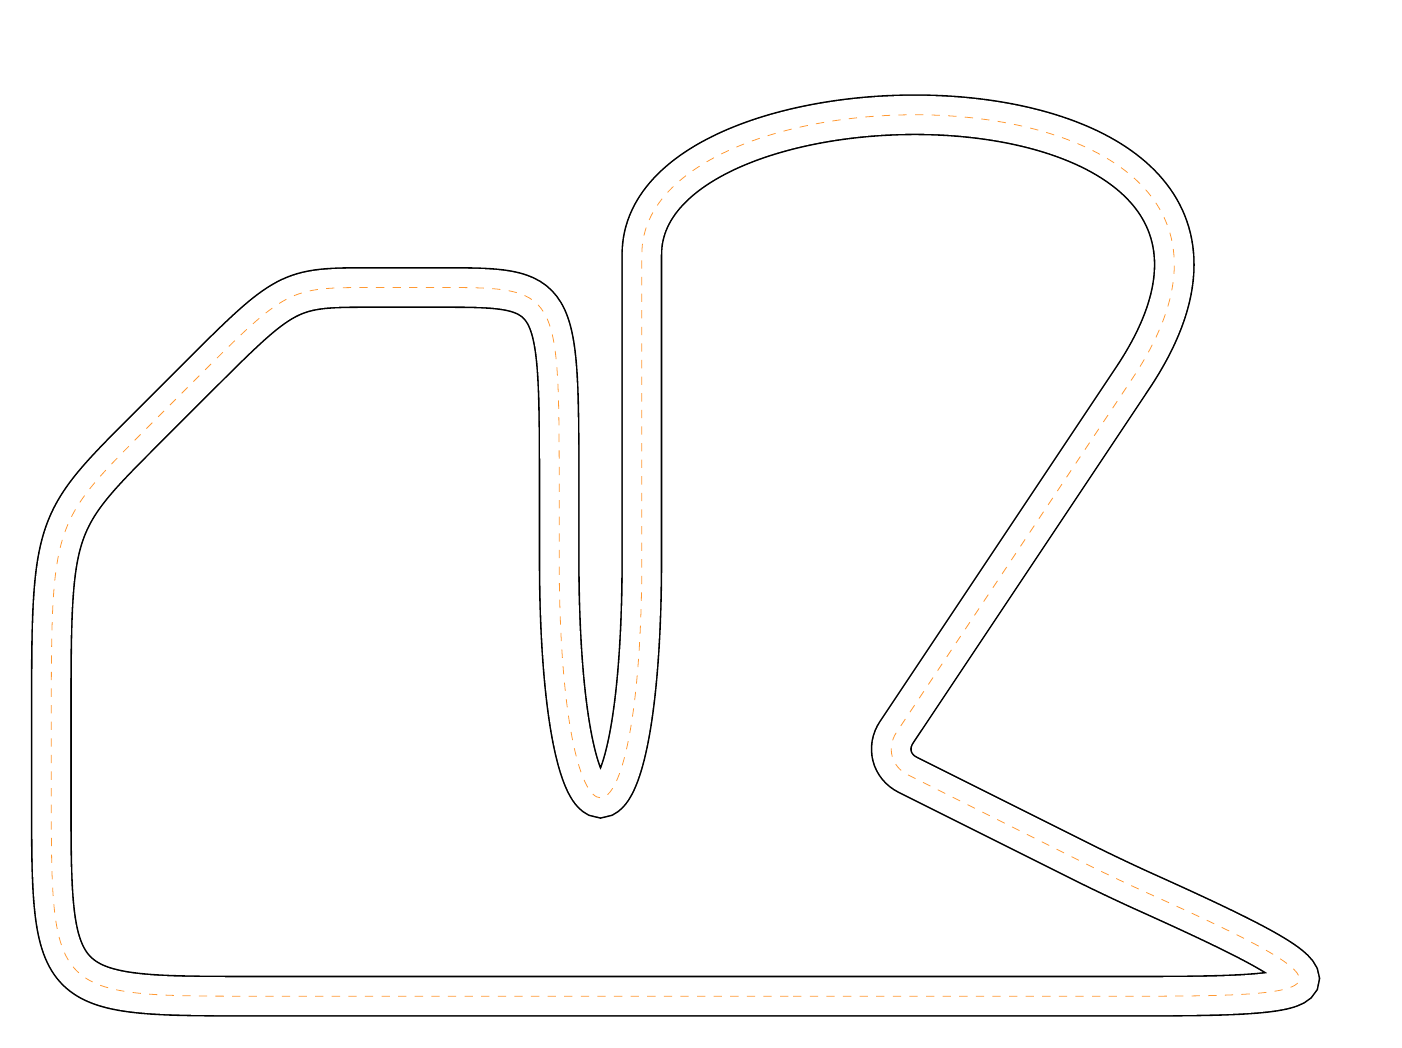
\begin{tikzpicture}[rounded corners=12pt, scale=1.5]
%\draw [black] plot [smooth cycle, tension=2] coordinates {(0, 0) (1, 0) (0.5, 0.5) (1,1) (0,1)};
%\track{black}{2}
%\track{red}{1.8}

%\draw[double=white, double distance=5mm, line width=0.8mm] plot [smooth cycle, tension=0.8] coordinates {(-2, -2)   (0, -1)  (2, -2) (1.5, 0) (2, 2) (-2, 2)};

%\draw[step=1cm,gray,very thin] (-5,-1) grid (5,8);

\draw[draw=white, double=white, double distance=5.2mm, line width=0.4mm] (0,0) -- (3,0) .. controls (5,0) and (5, 0.1) .. (3, 1) -- (1, 2) -- (3, 5)  .. controls (5, 8) and (-1,8) .. (-1, 6) -- (-1, 4) .. controls (-1, 1) and (-1.7, 1) .. (-1.7, 4) .. controls (-1.7, 6) and (-1.7, 6) .. (-3, 6) .. controls (-4, 6) and (-4, 6) .. (-5, 5) .. controls (-6, 4) and (-6, 4) .. (-6, 2) .. controls (-6, 0) and (-6, 0) .. (-4, 0) -- cycle;

\draw[draw=black, double=white, double distance=4.8mm, line width=0.2mm] (0,0) -- (3,0) .. controls (5,0) and (5, 0.1) .. (3, 1) -- (1, 2) -- (3, 5)  .. controls (5, 8) and (-1,8) .. (-1, 6) -- (-1, 4) .. controls (-1, 1) and (-1.7, 1) .. (-1.7, 4) .. controls (-1.7, 6) and (-1.7, 6) .. (-3, 6) .. controls (-4, 6) and (-4, 6) .. (-5, 5) .. controls (-6, 4) and (-6, 4) .. (-6, 2) .. controls (-6, 0) and (-6, 0) .. (-4, 0) -- cycle;

\draw[draw=orange!80, dashed, line width=0.1mm] (0,0) -- (3,0) .. controls (5,0) and (5, 0.1) .. (3, 1) -- (1, 2) -- (3, 5)  .. controls (5, 8) and (-1,8) .. (-1, 6) -- (-1, 4) .. controls (-1, 1) and (-1.7, 1) .. (-1.7, 4) .. controls (-1.7, 6) and (-1.7, 6) .. (-3, 6) .. controls (-4, 6) and (-4, 6) .. (-5, 5) .. controls (-6, 4) and (-6, 4) .. (-6, 2) .. controls (-6, 0) and (-6, 0) .. (-4, 0) -- cycle;


\end{tikzpicture}
\end{document}